\documentclass[12pt,epsf,makeidx,oneside]{book}

%\input{vhdllisting.tex}

\usepackage[a4paper, total={6.5in, 10in}]{geometry}
\usepackage{subfigure}
\usepackage{epsfig}
\usepackage{graphicx}
\usepackage{listings}
\usepackage{xcolor}
\usepackage{color}

\usepackage{url}
\usepackage{graphicx}
\usepackage{listings}
\usepackage{hyperref}
\usepackage[absolute,overlay]{textpos}
\usepackage{wasysym}
\usepackage[font=small,labelfont=bf]{caption}
\usepackage{adjustbox}
\usepackage{multirow}
\usepackage{enumitem}

\graphicspath{{./}{./img/}}  

\begin{document}

\lstset{backgroundcolor=\color{lightgray}}

\setcounter{tocdepth}{3}
\setcounter{secnumdepth}{3}

\begin{titlepage}
  \begin{center}
    \vspace*{4cm}
    \Huge{\bf Lab Workbook}\\
    \Large{SS 2022}\\
    \vspace{1.5cm}
    \Huge{Industrial Hardware Verification}\\
    \vspace{3cm}
    \Large{
      Jakob Lechner \\
      Markus Ferringer \\
    }
    \vspace*{3cm}
    \Huge{
      Part 1: VHDL \& FLI \& OSVVM
    }
  \end{center}
\end{titlepage}

\tableofcontents

\chapter*{Lab Mode}
\begin{itemize}[noitemsep]
  \item You have to elaborate these exercises on your own. This lab part is {\bf not} a team effort.
  \item We provide stubs containing basic templates for you which are to be extended with your implementations
  \item Questions are to be ansered in the respective source-files of the corresponding exercise. Just add appropriate comments at the end
  \item If you provide additional files (eg, images, diagrams, tables as part of your answers to questions) please make a note in the source files so that we don't miss anything
  \item Additional files must be located in the folder corresponding to the exercise
  \item I strongly recommend to read through an entire task before starting with the implementation (including the questions section). You will sometimes find hints later that might simplify things
  \item Once done with all exercises, please execute {\tt ./make.sh clean} in each folder, zip everything ({\tt ex1 - ex7}) and submit it via TUWEL
\end{itemize}

\chapter{Installation}
This chapter explains how to install the necessary software and get the lab exercises. You can do most of the work on your own personal computer. Only when special simulator features (such as Code Coverage or PSL) are needed, you need to work on the lab machines in order to use the respective licenses. 

Both Windows and Linux should work, although Linux will be less effort to set up. While it is possible to use Microsoft Windows (eg., using CygWin or WSL), these instructions focus on Linux-based systems like Ubuntu. 

You don't need to install any software on the Lab Workstations, everything you need is preinstalled.

\section{ModelSim/QuestaSim}
  On the lab workstations, everything is set up. Should you want to work with your personal equipment, you need to download the simulator first:
  \begin{enumerate}[noitemsep]
    \item Download ModelSim-Intel FPGA Starter Edition. Sounds easy? Well...
    \item https://www.intel.com/content/www/us/en/software/programmable/quartus-prime/model-sim.html
    \item You need to register. It's free, but it's a requirement.
    \item Once registered, sign in; Unfortunately, the site is not well structured...
    \item Click on your Avatar (top right) and choose ``Intel FPGA Design Software Download Center''
    \item On the left, under ``Additional Software'' choose ``Intel FPGA Simulation Tools'' and then ``Questa-Intel FPGA Starter Edition''
    \item From the list, choose the one for your platform. Use the latest version, eg ``Intel Quartus Prime Pro Edition Design Software Version 21.4 for Windows''
    \item Now click ``Individual Files'' as the complete download is over 70GB
    \item Download ``Questa-Intel FPGA Edition (includes Starter Edition)'' and ``Questa-Intel FPGA Edition (includes Starter Edition) Part 2''. It's still over 10GB.
    \item Install the software
  \end{enumerate}

  The free version has a couple of restrictions, so for some exercises you have to use the lab workstations.
  \begin{itemize}[noitemsep]
    \item Reduced performance (which will not be an issue, though)
    \item No support for code coverage $\rightarrow$ use lab workstations
    \item No support for PSL $\rightarrow$ use lab workstations
  \end {itemize}

\section{C Compiler}
  For the FLI examples you need a C compiler. Under Linux, {\tt gcc} is just perfect. Under Windows, I used {\tt mingw32}. Please notice that you need a 32 bit compiler (or one that can comile in 32 bit mode using a switch like {\tt -m32}).
  It might also be necessary to install 32 bit support first, which can be done with 
  \begin{itemize}
    \item (Ubuntu): {\tt sudo apt-get install libc6-dev-i386}
    \item (CentOS): {\tt sudo yum install glibc-devel.i686 }
  \end{itemize}

  {\bf Remark}: At the time of writing (30.03.2022) the Lab Workstations have not installed 32 bit support. The lab admin is informed, and it should be available soon. I will keep you informed via the Forum. Thoses exercises can also be 
  run on you personal equipment, so lab access is not a requirement.

\section{Source Code}
  We prepared a framework for you which contains
  \begin{itemize}[noitemsep]
    \item OSVVM (in a separate folder)
    \item Exercises (each in a separate folder)
    \item A suitable {\tt make.sh} (one for each exercise)
    \item Stubs for all the exercises (containing basic templates where you can fill in your solution)
    \item The entire source-code needed for all exercises
  \end {itemize}

  You can download the execises via TUWEL. It will be available after the respective lectures.

  \vspace*{0.7cm}

  {\bf Remark for Windows Users: } The {\tt make.sh} files are symbolic links, which are not supported in Windows. If your make files don't work or are empty,
  try to copy the original {\tt make.sh} from the root-folder into the respective exercise folder.

\section{Compilation}
  Each exercise is located in a separate folder. There is a {\tt make.sh} file which supports the following targets. Please notice that this
  is not a regular Makefile, but rather a shell script named {\tt make.sh}. I prefer this over Makefiles.
  \begin{itemize}[noitemsep]
    \item {\tt ./make.sh clean}: Cleans up temporary files and compiled libraries
    \item {\tt ./make.sh sim}: Compiles the exercise's code, then executes the simulation. When called the very first time (or after a {\tt make.sh clean}), OSVVM is compiled.
    \item {\tt ./make.sh gui}: Opens the ModelSim/QuestaSim GUI and sources the OSVVM scripts, so you can use them right away
  \end{itemize}
  You need to provide the path to your / the lab's ModelSim/QuestaSim binary. In the root folder (the one that contains OSVVM and all 
  exercises) there is a file called {\tt settings.make}. Open it and edit the {\tt MODELSIM\_PATH} variable according to your setup.
  If ModelSim is available through your {\tt PATH} variable, just keep the default assignment {\tt MODELSIM\_PATH=vsim}.

  For the FLI example, you also need to provide the path to ModelSim's {\tt include} folder. Just edit the {\tt compile.sh} script accordingly. Depending on your setup,
  you might also need to change the C compiler used. There is a {\tt compile\_win.bat} for Windows, but you need to update the paths as well.

\section{Editor}
  Of course, you can use any editor you like. However, it will be more efficient (and way less frustrating) if you are using a good editor which is capable of
  understanding VHDL, and which offers at least some degree of support (like parameter help, tooltips, code completion, etc.). You have to deal with a lot
  of packages and libraries, and 100s of functions, procedures, and datatypes. You should use all the support you get from a good IDE.

  As I have written my own VHDL editor (an extension for Visual Studio Code), I will of course recommend this IDE to you :-) VS Code is Open Source and thus for free,
  and I will provide you with a license for my extension (it will be included in the lab exercises, you don't have to worry about it).

  \begin{itemize}[noitemsep]
    \item Download and install VS Code from \url{https://code.visualstudio.com/}
    \item Open VS Code ({\tt code} in the terminal)
    \item On the left side, open the {\tt Extensions} view
    \item In the search field, enter {\tt VHDL for professionals} (V4P)
    \item Select {\tt VHDL for Professionals} from the results, and click the {\tt install} button
    \item If requested, restart VS Code
    \item Open file {\tt workspace.code-workspace} which is located in the root folder of the provided zip file
  \end{itemize}

  All (VHDL-based) exercises come with a preconfigured VS Code workspace. Just open it in VS Code, and you are set to go. All the OSVVM libraries, functions, types, etc. are at your disposal. The license for V4P will also be part of the workspace.

    
%%%%%%%%%%%%%%%%%%%%%%%%%%%%%%%%%%%%%%%%%%%%%%%%%%%%%%%%%%%%%%%%%%%%%%%
%%% VHDL                                                            %%%
%%%%%%%%%%%%%%%%%%%%%%%%%%%%%%%%%%%%%%%%%%%%%%%%%%%%%%%%%%%%%%%%%%%%%%%
\chapter{VHDL}

%%%%%%%%%%%%%%%%%%%%%%%%%%%%%%%%%%%%%%%%%%%%%%%%%%%%%%%%%%%%%%%%%%%%%%%
\section{Exercise 1: Attributes}

\subsection{Task 1 [1 Point]}
  Write a function {\tt ColorToString(pos: integer) return string} with the following properties:
  \begin{itemize}[noitemsep]
    \item The function shall take an integer parameter which specifies the ``index'' of the enum-value in type {\tt ColorT} 
    \item If the index is invalid, the function shall call {\tt Alert()} with an appropriate error message and return {\tt ``OutOfRange''}
    \item If the index is valid, the string representation of the color at position {\tt pos} shall be returned
    \item The function shall work without modification even if colors are added or removed to/from {\tt ColorT}
    \item In the main process {\tt stimuli\_p}, add some calls to {\tt ColorToString()} and see if it works
    \item Example:
    \begin{lstlisting}[language=VHDL,gobble=6,numbers=left]
      architecture beh of ent is
        type ColorT is (Red, Green, Blue);
        ...
      begin
        -- Expected output: ``green''
        report ColorToString(1) severity note; 
      end architecture;
    \end{lstlisting}
    \item Answer the following questions (directly in the source file as comment):
    \begin{itemize}
      \item What is the result of {\tt ColorT'leftof(Red)}, {\tt ColorT'succ(Yellow)}, {\tt ColorT'val(5)}? 
      \item How does the simulator handle those situations?
    \end{itemize}
  \end{itemize}

\subsection{Task 2 [1 Point]}
   Write a function {\tt ColorsToList() return string}
  \begin{itemize}[noitemsep]
    \item The function shall return a comma-separated list of all enumeration fields that are part of the {\tt ColorT} type
    \item Example:
    \begin{lstlisting}[language=VHDL,gobble=4,numbers=left]
      architecture beh of ent is
        type ColorT is (Red, Green, Blue);
        ...
      begin
        -- Expected output: "AllEnums: red, green, blue"
        report "AllEnums: " & ColorsToList() severity note; 
      end architecture;
    \end{lstlisting}
    \item Hints
    \begin{itemize}[noitemsep]
      \item Use dynamic strings: Define a string access type (don't use {\tt textio.line})
      \item Make sure the function handles one-element enums
      \item The function shall work without modifications even if the {\tt ColorT} type is changed
    \end{itemize}
    \item Answer the following questions (directly in the source file as comment):
    \begin{itemize}[noitemsep]
      \item During implementation, did you run into segmentation faults? Why?
      \item Does your implementation contain memory leaks? If so, explain why.
      \item If there are memory leaks, can you imagine a way to avoid them?
      \item Especially for this simple exercise, can you imagine a way to find out if the implementation contains memory leaks?
    \end{itemize}
  \end{itemize}

%%%%%%%%%%%%%%%%%%%%%%%%%%%%%%%%%%%%%%%%%%%%%%%%%%%%%%%%%%%%%%%%%%%%%%%
\section{Exercise 2: Transactions}

\subsection{Task 1 [1 Point]}
\begin{itemize}[noitemsep]
  \item We provide a very simple state machine that is controled by process {\tt stimuli\_p}. Every 20 clock cycles, the state is advanced.
  \item Take a look at process {\tt state\_p}: Depending on the state, signal {\tt output} is modified in different ways
  \item Implement a process {\tt event\_count\_p} that increments {\tt eventCounter} every time {\tt output} changes
  \item Implement a process {\tt trans\_count\_p} that increments {\tt transCounter} every time a transaction occurs on {\tt output}
  \item Answer the following questions (directly in the source file as comment):
  \begin{itemize}[noitemsep]
    \item Explain the difference between the two processes and how they are triggered
    \item Is there a difference between the assignment statements of the states {\tt Idle, NotAffected, Keep}?
  \end{itemize}
\end{itemize}

\subsection{Task 2 [1 Point]}
\begin{itemize}[noitemsep]
  \item Enhance process {\tt stimuli\_p} such that the testbench self-checks the counter values
  \item After each call to {\tt WaitForClock()} in {\tt stimuli\_p}, add {\tt AffirmIfEqual(actual, expected, message)} statements. Just hardcode the expected values.
  \item Open up the GUI ({\tt ./make.sh gui}), and execute {\tt build project.pro}
  \item Now add all the signals to the waveform viewer. Save the waveform (filename {\tt wave.do})
  \item Restart the simulation with {\tt build project.pro}
  \item Inspect the results in the waveform viewer. If there is a {\tt wave.do} it is automatically opened.
  \item Answer the following questions (directly in the source file as comment):
  \begin{itemize}[noitemsep]
    \item How can you make {\tt output'transaction} visible in the waveform viewer?
    \item Can you imagine scenarios where {\tt sig'transaction} is actually useful? Why would we want events if there is no change of data?
    \item Why is {\tt stimuli\_p} reacting on the falling edge, while {\tt state\_p} triggers on the rising edge?
  \end{itemize}
\end{itemize}

%%%%%%%%%%%%%%%%%%%%%%%%%%%%%%%%%%%%%%%%%%%%%%%%%%%%%%%%%%%%%%%%%%%%%%%
\section{Exercise 3: Delay Modes}
\begin{center}
  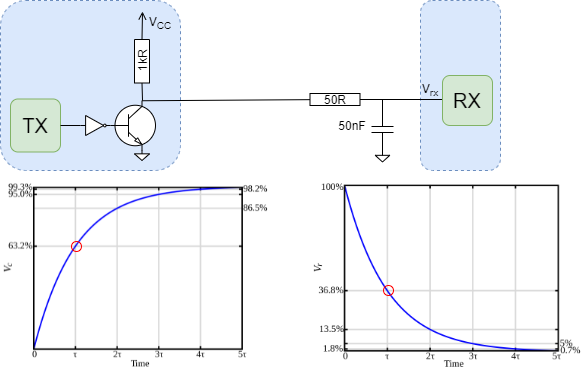
\includegraphics[width=0.6\textwidth]{transmission}
\end{center}

\subsection{Task 1 [2 Points]}
Consider the electrical transmission line in the figure above.
\begin{itemize}[noitemsep]
  \item Model the physical transmission line in VHDL
  \begin{itemize}[noitemsep]
    \item Output is open collector with a $1k\Omega $ pull-up resistor
    \item The transmission line itself has an impedance of $50\Omega$ and a parasitic capacitance of $50nF$ at the receiver
    \item Assume that the delay from TX to RX is $23ns$
    \item Assume that RX recognizes $V_{rx}\ge0.632V_{cc}$ as logical 1 ($1\tau$ as indicated)
    \item Assume that RX recognizes $V_{rx}\le0.368V_{cc}$ as logical 0 ($1\tau$ as indicated)
    \item If $V_{rx}$ is between these two thresholds, the internal logic value does not change
    \item The transistor can be modeled as ideal switch
    \item You can assume that signal transitions are far enough separated so that they don't interfere with each other
  \end{itemize}
  \item Answer the following questions (directly in the source file as comment):
  \begin{itemize}[noitemsep]
    \item Given this specification, what is the maximum frequency that can safely be transmitted?
    \item In the analog world... 
    \begin{itemize}[noitemsep]
      \item how do typical transitions on the wire look like? (just add a photo or something adequate of a hand-written diagram)
      \item how does an eye diagram look like? (just add a photo or something adequate of a hand-written diagram)
    \end{itemize}
    \item What happens in your simulation if the maximum frequency is exceeded?
    \item What would happen on an actual transmission line if the frequency was exceeded?
  \end{itemize}
\end{itemize}

\subsection{Task 2 [1 Point]}
\begin{center}
  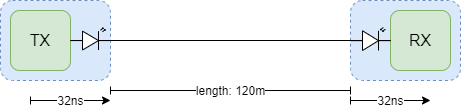
\includegraphics[width=0.6\textwidth]{optical}
\end{center}
Now model an optical transmission line with the following properties
\begin{itemize}[noitemsep]
  \item Fiber length is 120m (speed of light is around 200000km/s in the optical medium)
  \item The laser's propagation time from electrical input to optical output is 32ns for both rising and falling edges
  \item After a transition on the input, the laser ignores all glitches on the input for 20 ns
  \item On the receive side, the optical detector has the same characteristics as the transmitter
  \item As the transmission line is quite long, you cannot longer assume that only one signal is transmitted at a time (i.e., a new transition can be sent before the last one has arrived)
  \item Hint: You will need an intermediate signal to combine {\tt inertial} and {\tt transport} delays
  \item Answer the following questions (directly in the source file as comment):
  \begin{itemize}[noitemsep]
    \item What is the rejection time of {\tt inerial} if you don't specify it explicitly?
    \item Can the rejection time be greater that the corresponding inertial delay?
    \item If modeled correctly, any \emph{glitches} on the input shorter than 20 ns are ignored. But what happens if a {\bf single} signal 
          transition happens within the rejection time and the signal then remains constant afterwards? Like so:\\
          {\tt tx <= '0' after 0 ns, '1' after 100 ns, '0' after 110 ns}\\
          (Your solution does {\bf not} need to solve this problem!)
  \end{itemize}
\end{itemize}


%%%%%%%%%%%%%%%%%%%%%%%%%%%%%%%%%%%%%%%%%%%%%%%%%%%%%%%%%%%%%%%%%%%%%%%
\section{Exercise 4: Advanced Data Types, Generics}
  \subsection{Task 1 [4 Points]}
  Your task is to implement a (singly) linked list in VHDL
  \begin{itemize}[noitemsep]
    \item The list shall be implemented as protected type inside package {\tt linked\_list}.
    \item The linked list shall be located in a generic package, which takes two generic parameters
    \begin{itemize}[noitemsep]
      \item {\tt type ElementT}: The type of the items that are stored in the list
      \item {\tt function ToStringF(item: ElementT) return string}: A function that converts an item to a string representation
    \end{itemize}
    \item This generic data type denotes the type of the elements that can be stored inside the list
    \item Implement the following functions/procedures:
    \begin{itemize}[noitemsep]
      \item {\tt function Count return integer}: Returns the number of elements in the linked list
      \item {\tt procedure AddLast(item: ElementT)}: Adds an element to the end of the list
      \item {\tt procedure AddFirst(item: ElementT)}: Adds an element to the front of the list
      \item {\tt function GetFirst return ElementT}: Returns the first element of the list
      \item {\tt function GetLast return ElementT}: Returns the last element of the list
      \item {\tt function GetAt(index: integer) return ElementT}: Return the i-th item of the list. The first item (head of list) has index 0.
      \item {\tt procedure RemoveAt(index: integer)}: Remove the i-th item from the list. The first item (head of list) has index 0.
      \item {\tt procedure AddAfter(index: integer; item: ElemetT)}: Adds the item after the i-th item in the list. The first item (head of list) has index 0.
      \item {\tt function Dump return string}: Returns a comma separated list of string representations of all items in the list (in the stored order, of course)
    \end{itemize}
    \item In case of invalid operations (eg, get a value from an empty list), create a log entry by calling {\tt Alert(...)}
  \end{itemize}

  \subsection{Task 2 [3 Points]}
  Your task is to implement a testbench which tests all the linked list (process {\tt stimuli\_p})
  \begin{itemize}[noitemsep]
    \item Instantiate the generic list, use {\tt PrimeRecT} as generic type and implement the ToString function for this data type
    \item Test all public subroutines that are part of the public interface
    \item Make sure that Statement Coverage is at 100\% (for the linked-list protected type)
    \item You can use the GUI (Tools - Coverage Report...) to generate annotated source files
    \item Attach the annotated source code (coverage report) to your submission
  \end{itemize}

%%%%%%%%%%%%%%%%%%%%%%%%%%%%%%%%%%%%%%%%%%%%%%%%%%%%%%%%%%%%%%%%%%%%%%%
%%%%%%%%%%%%%%%%%%%%%%%%%%%%%%%%%%%%%%%%%%%%%%%%%%%%%%%%%%%%%%%%%%%%%%%
%%%%%%%%%%%%%%%%%%%%%%%%%%%%%%%%%%%%%%%%%%%%%%%%%%%%%%%%%%%%%%%%%%%%%%%

% wavedrom source
%{ signal: [
%  { name: "clk",      wave: 'p.......' },
%  { name: "addr",     wave: 'x2..xx2x'},
%  { name: "byte_ena", wave: 'x2..xx2x'},
%  { name: "read",     wave: '01..0...' },
%  { name: "readdata", wave: 'x..2x...' },
%  { name: "write",    wave: '0.....10' },
%  { name: "writedata",wave: 'x.....2x' },
%]}
\chapter{OSVVM}
  \section{Exercise 5: OSVVM Verification Unit}
  \subsection{Task 1 [4 Points]}
  Your task is to implement a Verification Unit for the Avalon Memory Mapped (AVMM) Bus. Your are
  implementing a master device, which can in turn control DUTs with memory mapped slave interfaces.
  Notice that this VU is already in preparation for the Verification Project, where you will need
  an AVMM master component.
  \begin{center}
    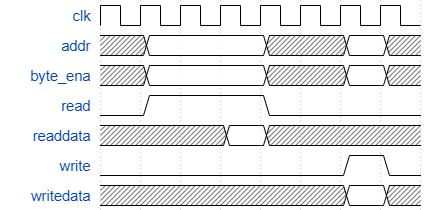
\includegraphics[width=0.6\textwidth]{avmm_timing}
  \end{center}
  \begin{itemize}[noitemsep]
    \item The read and write timing is shown in the image. This timing is fixed, and need not be configurable. The shown waveform corresponds to {\tt writeWaitTime=0} and {\tt readWaitTime=2}
    \item It is not necessary to support simultaneous read and write access.
    \item The interface uses byte enables. 
    \item It does not use WaitRequest, and ReadDataValid (the latter is implicit due to timing). You don't have to support bursts. You don't have to support pipelined reads / writes (i.e., just one read/write at a time, until the entire sequence is finished)
    \item There is a template package file which contains definitions of the public interface of the VU
    \begin{itemize}[noitemsep]
      \item Implement the subroutine bodies of the respective header definitions
      \item Use the AddressBusTransactionRecT data structure, it is well suited for this task
      \item There are a couple of predefined OSVVM subroutines (eg, {\tt send}) which are already performing 
            lots of the necessary steps. Use them, or review them to adapt you own implementation
      \item You might want to take a look at OSVVM's UART and AXI implementation for reference
    \end{itemize}
    \item There is the main VU's source file which already contains a basic skelton of the VU
    \begin{itemize}[noitemsep]
      \item For simplicity, both reading and writing shall be blocking - so there is no need to implement FIFOs to buffer incoming or outgoing data transactions
      \item Implement the VU. As there are only blocking operations, it is simplest to just use one process which does all the work (read data, write data)
    \end{itemize}
  \end{itemize}

  \subsection{Task 2 [3 Points]}
  Your task is to implement a basic (directed) testbench for your VU
  \begin{itemize}[noitemsep]
    \item Test all the functions of the public interface
    \begin{itemize}[noitemsep]
      \item Use an address-width of 5 bits, and a data-width of 16 bits
      \item Use a scoreboard. For each call to one of the public functions, create the respective expected waveforms on the avalon bus and store then in the scoreboard.
      \item Write a process that monitors the bus; put the observed waveforms in the scoreboard for checking.
      \item For this exercise, it is good enough to hardcode the waveforms. Usually, you should of course implement a reference model.
    \end{itemize}
    \item Reach 100\% statement coverage for the main VU design, and the public package
  \end{itemize}

%%%%%%%%%%%%%%%%%%%%%%%%%%%%%%%%%%%%%%%%%%%%%%%%%%%%%%%%%%%%%%%%%%%%%%%

\section{Exercise 6: Constrained Random Testing}
\subsection{Task 1 [4 Points]}
{\scriptsize
  \begin{center}
    \begin{tabular}{|c|c|c|c|c|c|c|c|c|}
      \hline
      Addr  & 7 & 6 & 5 & 4 & 3 & 2 & 1 & 0 \\
      \hline
      0 & IE  & IF  & \multicolumn{5}{| c |}{-}  &  RST   \\
      \hline
      1 &  \multicolumn{4}{| c |}{NAME} & \multicolumn{4}{| c |}{CHK}   \\
      \hline
      2 &  \multicolumn{4}{| c |}{-} & \multicolumn{4}{| c |}{ID}   \\
      \hline
      3 & \multicolumn{8}{| c |}{CNT}  \\
      \hline
    \end{tabular}
    \\
    \begin{tabular}{|c|c|c|c|}
      \hline
      Name & Access & Default & Remarks \\
      \hline
      RST & R/W & 0 & Write 1 to reset all registers to their default. The field auto-clears to zero. \\
      \hline
      IF & R & 1 & Auto-clears when read. Then remains 0 until RST \\
      \hline
      IE & R/W & 0 & \\
      \hline
      CHK & R & 1010 & NAME xor ID \\
      \hline
      NAME & R/W & 0000 & \\
      \hline
      ID & R & 1010 & \\
      \hline
      CNT & R & 00000000 & Increments by one with each clock cycle. Overflows to 0 when maximum is reached \\
      \hline
    \end{tabular}
  \end{center}
}
  Your task is to use constrained random testing in combination with functional coverage to test a given DUT.
  \begin{itemize}[noitemsep]
    \item The DUT is a simple register interface
    \begin{itemize}[noitemsep]
      \item There is no internal state other than the registers directly accessible through the memory mapped interface
      \item The register description is shown in the table
      \item Read/Write access timings are the same as for the previous exercise, byteenables are ignored. 
    \end{itemize}
    \item Use the VU implemented in the previous exercise to save time. Alternatively, you can implement all the bit-banging again, neglecting the advantages of code reuse :-)
    \item It is not necessary to test the bus protocol itself. Limit your testing to sending valid read/write requests.
    \item Use OSVVM's functional coverage capabilities to specify cover points for the defined register fields
    \begin{itemize}[noitemsep]
      \item Eg, all addresses have been read from
      \item Eg, all writable fields have been written to
      \item Eg, all writeable fields have been read from after they have been written to, etc.
      \item ...
    \end{itemize}
    \item The DUT has some undocumented ``features/bugs''. Can you find them using constrained random testing?
  \end{itemize}

%%%%%%%%%%%%%%%%%%%%%%%%%%%%%%%%%%%%%%%%%%%%%%%%%%%%%%%%%%%%%%%%%%%%%%%
%%%%%%%%%%%%%%%%%%%%%%%%%%%%%%%%%%%%%%%%%%%%%%%%%%%%%%%%%%%%%%%%%%%%%%%
%%%%%%%%%%%%%%%%%%%%%%%%%%%%%%%%%%%%%%%%%%%%%%%%%%%%%%%%%%%%%%%%%%%%%%%
\chapter{FLI}
\section{Exercise 7: FLI}
\subsection{Task 1 [3 Points]}
  Your task is to implement a Mandelbrot Set renderer in VHDL and C, and compare the performance of both variants
  \begin{itemize}[noitemsep]
    \item We prepared a basic framework for you to easily compile C code and use it from within vhdl
    \begin{itemize}[noitemsep]
      \item Use {\tt compile.sh} to compile for linux. It should work right way
      \item Use {\tt compile\_win.bat} to compile for windows. You need to update the path to your compiler. Might make problems...
    \end{itemize}
    \item Calculcating the Mandelbrot set is quite easy. Google is your friend.
    \item In short, given a complex number $c$, calculcate $z_{n+1}=z_n^2+c$ with $z_0=0$. If $z_n$ evaluates to ($|z_n|>2.0$), the point is not part of the set. 
    \item We are counting and ``colorizing'' $n$, i.e. the number of iterations we need until the point escapes. We also need to define an upper limit for $n$
          for which we consider the point to belong to the set. We define it to be 200.
    \item Implement the following functions / procedures in C
    \begin{itemize}[noitemsep]
      \item {\tt function GetTimeC return string}: Write a C function to get the current time (including seconds) as string. We need this for performance measurement.
      \item {\tt procedure OneStepC(zr, zi, cr, ci: real; or, oi: out real)}: Write a function that performs one step of the mandelbrot calculation $o=z^2+c$
      \item {\tt function IterateC(x, y: real) return integer}: Calculate the Mandelbrot escape value for the given (complex) point (x, y). Don't do more than 200 iterations. 
            Stop if the magnitude of the complex vector exceeds 2.0
      \item Take a look at the data type mapping table in the slides to learn how to pass certain data types back and forth via FLI
    \end{itemize}
    \item Define the subroutine defintions in VHDL and mark them as foreign.
    \item Implement the same functions and procedures in VHDL. You need to give them distinct names because we want to use both VHDL and C functions at the same time. Use the {\tt ieee.math\_complex.Complex} data type.
    \item Run the following simulations and record the execution times:
    \begin{itemize}[noitemsep]
      \item Everything VHDL: {\tt Image} calls {\tt Iterate} calls {\tt OneStep}
      \item {\tt Image} calls {\tt Iterate} calls {\tt OneStepC}
      \item {\tt Image} calls {\tt IterateC} (calls {\tt OneStepC} directly in C)
    \end{itemize}
  \end{itemize}

\end{document}